\section{Formalization of the Method}
\label{sec:theory}

\begin{comment}
The main idea that we present in this research is as follows. The MIVCs are MUSs (Minimal Unsatisfiable Subsets) of a constraint system that normally consists of the assumptions and guarantees of system components and the negation of the safety property of interest. The MCSs (Minimal Correction Sets), the sets that contain the minimal ``correction" of the infeasible constraint system, can then be obtained from all MUSs. Here is the key idea that we present: if the constraint system is defined to take into account fault activation literals as well as component contracts, these MCSs and the information they contain can be transformed into MinCutSets. A small example will illustrate this point nicely. 

Let a constraint system $C$ consist of guarantees $g_1$, $g_2$, fault activation literals constrained to $false$, $\neg f_1$, $\neg f_2$, and the safety property $P$ also constrained to $false$, $\neg P$. 
\begin{equation}
    C = \{\neg f_1, \neg f_2, g_1, g_2, \neg P\}
\end{equation}

Now, since we assume that the nominal model proves, it is no surprise that $C$ is UNSAT. (The guarantees are valid, no faults occur, and we want to prove the negation of the safety property.) The MIVC algorithm returns the minimal unsatisfiable subsets, say $MIVC_1 = \{\neg f_1, g_2\}$ and $MIVC_2 = \{\neg f_2\}$. Let us focus on $MIVC_1$. This can be understood in two ways: (1) $MIVC_1$ is a proof core: if $f_1$ does not occur and $g_2$ holds, then the property $P$ can be proven, or (2) $MIVC_1$ is a minimal unsatisfiable subset: it cannot be the case that $f_1$ does not occur and the guarantee $g_2$ holds. 

Next we look at the MCSs for this example:
\begin{center}
    $MCS_1 = \{\neg f_1, \neg f_2\}$,
    $MCS_2 = \{\neg f_2, g_2\}$
\end{center}

This means that $C \setminus MCS_1$ is SAT. So by removing those constraints from $C$, we get a SAT constraint system: $C \setminus MCS_1 = \{f_1, f_2, g_1, g_2, \neg P\}$. When both faults $f_1$ and $f_2$ are active, $\neg P$ can be proven; i.e., this is a cut set for $\neg P$. The minimality of the MCS gives the minimality of the cut set. 
\end{comment}









Throughout the remainder of this section, we provide the formal background necessary to show how this approach works.

In the case of a nominal model augmented with faults, a constraint system can be defined as follows. Let $F$ be the set of all fault activation literals defined in the system and $G$ be the set of component contracts (guarantees of component output behavior). 

\begin{definition}Let $C = \{C_1,C_2,...,C_n\}$ be a constraint system such that for $i \in \{1,...,n\}$, $C_i$ has the following constraints for any $f_j \in F$ and $g_k \in G$ with regard to the top level property $P$: 
\begin{center}
$C_i \in \left\{ \begin{array}{ll}
	f_j :&  false\\
	g_k :& true\\
	P :& false\\
\end{array}\right.$	
\end{center}
\label{def:constraintsystem}
\end{definition}

\begin{comment}
The \aivcalg algorithm collects all minimal unsatisfiable subsets of a given transition system in terms of the \textit{negation} of the top level property~\cite{Ghassabani2017EfficientGO,bendik2018online}. Assuming that the nominal model proves (no faults are active), it is not surprising that the guarantees and the negation of the safety property is UNSAT. The MUSs are the minimal explanation of the infeasibility of this constraint system; equivalently, these are the minimal sets of model elements necessary for proof of the safety property.

We utilize this algorithm by providing not only component contracts as model elements, but also fault activation literals constrained to \textit{false}, i.e., the faults are inactive. Thus the resulting MIVCs (MUSs) will contain the required contracts and constrained fault activation literals necessary to prove the safety property. 

Because of the duality between MUSs and MCSs, all MCSs can be obtained by finding the hitting sets of all MUSs. The MCS can be seen to correct the infeasibility of the constraint system and provides the minimal such correction. By removing the constraints from $C$ that are found in any MCS, $C$ becomes satisfiable. In terms of the constraint system that includes fault activation literals, by \textit{activating} the faults in the MCS and \textit{violating} the contracts in the MCS, we can prove the \textit{negation} of the property $P$. This is the precise information we require to find the minimal cut sets of a system. If the contracts in the MCS are replaced with the faults that cause its violation, the MCS is transformed into a MinCutSet. A high level summary of the steps of this transformation are shown in Figure~\ref{fig:trans}. 

\begin{figure*}[h!]
	%\vspace{-0.1in}
	\begin{center}
		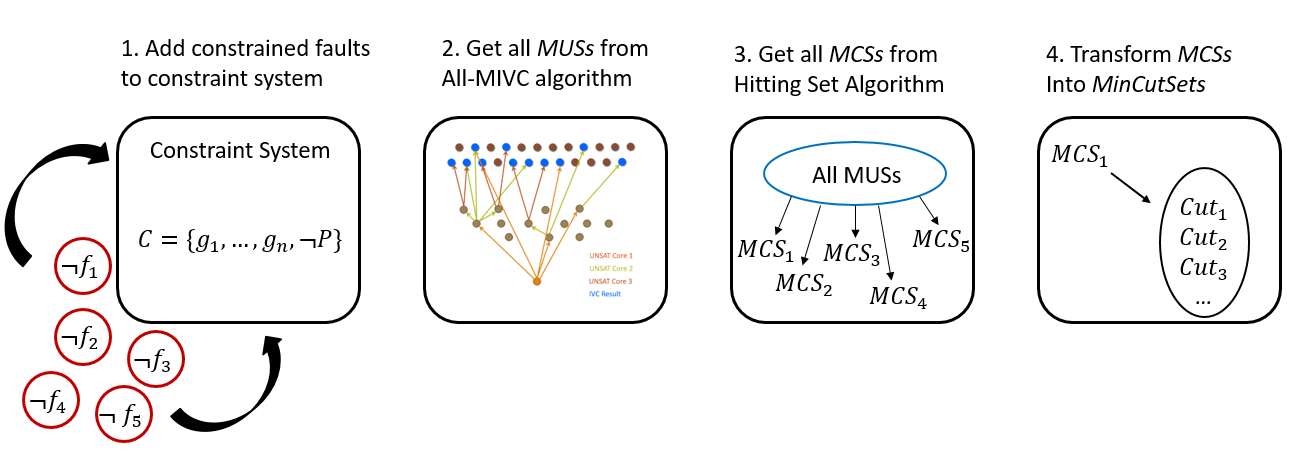
\includegraphics[width=0.8\textwidth]{images/highLevelIdea.PNG}
	\end{center}
	\caption{Steps of the Transformation Process}
	\label{fig:trans}
\end{figure*}

\danielle{End of copy/paste.}

\end{comment}
The theory regarding MIVCs and the duality of MUSs with MCSs has been established~\cite{GhassabaniGW16,Ghassabani2017EfficientGO,liffiton2016fast}. The MCSs are transformed into Minimal Cut Sets according to the following theoretical results. We assume that the nominal model proves a safety property $P$. Then since the nominal model consists of all its component contracts, $G$, and all faults constrained to false, $F$, we can say that $F \cup G$ satisfies $P$ and the constraint system $C = F \cup G \cup \{\neg P\}$ is UNSAT for disjoint sets $F$ and $G$.

Let the set $\overline{MCS}$ be an MCS with all constraints removed.

\begin{lemma}
$\overline{MCS}$ satisfies $\neg P$.

%If the only elements of a MCS are constrained faults, these unconstrained faults are a minimal cut set.
\begin{proof}
Let $\overline{MCS}$ consist of the elements of MCS with constraints removed and let $C = E \cup \{\neg P\}$ for all model elements $E$ (i.e., $E = F \cup G$). Since $C$ is UNSAT, clearly $E$ does not satisfy $\neg P$. \\

Since $MCS \subseteq E$, we can further decompose $E$. Let the set $L_E$ be all elements of $E$ that are not found in $MCS$; the leftover elements. Then $E = L_E \cup MCS$ for disjoint sets $L_E$ and $MCS$. \\

It follows that since $E$ does not satisfy $\neg P$, we know that neither $L_E$ nor $MCS$ satisfies $\neg P$.\\ 

But we also know by the definition of $MCS$ that $C \setminus MCS$ satisfies $\neg P$ (i.e., removing all constraints from the elements in $C$ that are found in the $MCS$ produces a satisfiable constraint system). \\

Let $\overline{MCS}$ be the MCS with all constraints removed. Then $C \setminus MCS$ can be represented as: $C = L_E \cup \overline{MCS} \cup \{\neg P\}$ which is satisfiable. \\

Since $L_E$ does not satisfy $\neg P$, it must be the case that $\overline{MCS}$ does satisfy $\neg P$.

\end{proof}
\label{lem:minCorrSet1}
\end{lemma}
\vspace{-2em}

In order to transform the MCS into a minimal cut set, any contracts found in the MCS must be replaced with faults that cause their violation. We show that making this replacement still satisfies $\neg P$.

\begin{lemma}
	Replacement of a contract $g \in \overline{MCS}$ with the faults that cause its violation satisfies $\neg P$.
	\begin{proof}
	Assume that there exists a $g \in G$ where $g \in MCS$. Given the assumption that $G \cup \{P\}$ is SAT (i.e., the nominal model proves), $\neg g$ can only occur by activation of faults. For the set of all faults in the system, $F$, let $F_G \subseteq F$ such that $F_G$ satisfies $\neg g$ and let $F_G$ be a minimal such set (i.e. $F_G$ is a minimal cut set for $g$). Replace $g \in \overline{MCS}$ with $F_G$; call this new set $MCS_{repl}$. By the assumption that $F_G$ satisfies $\neg g$ and lemma 1, the result is immediate.
	\end{proof}
	\label{lem:corrSet}
\end{lemma}
\vspace{-2em}

\begin{lemma}
$MCS_{repl}$ is minimal.
\begin{proof}
The minimality follows directly from the definition of MCS. 

\end{proof}
\label{lem:minCorrSet}
\end{lemma}
\vspace{-2em}
Once all replacements have been made, the set $MCS_{repl}$ contains only faults. Since $MCS_{repl}$ satisfies $\neg P$, these unconstrained faults are a cut set for $\neg P$. Thus, iterative replacement of each contract in an MCS with a minimal cut set of that contract and removal of all constraints of the elements in MCS results in minimal cut set. 

\begin{theorem}
A minimal correction set can be transformed into a minimal cut set.
\begin{proof}
Result follows directly from lemmas 1-3.
\end{proof}
\end{theorem}

%For more information on the implementation of these theoretical results, see section~\ref{sec:algs}.





